% !TeX program = xelatex
% !TeX encoding = UTF-8
% !TeX TXS-program:compile = txs:///xelatex | txs:///xelatex
\documentclass[aspectratio=169, table, 12pt]{beamer}
% Preamble bersama seluruh slide mata kuliah ini.
% Dipanggil dari slides/sessionXX/sessionXX.tex tepat sesudah baris
% \documentclass[aspectratio=169, table, 12pt]{beamer}
% Paket tambahan yang hanya dibutuhkan satu sesi ditulis di berkas sesi itu.

\usepackage{colortbl}
\usepackage{xcolor}
\usepackage{listings}
\usepackage{tabularx}
\usepackage{booktabs}
\usepackage{tikz}
\usepackage{pgfplots}
\pgfplotsset{compat=1.18}
\usetikzlibrary{arrows.meta, positioning, calc, fit, shapes.geometric,
	shapes.multipart, backgrounds, matrix, chains, trees}

\makeatletter
\def\input@path{{../theme/}}
\makeatother
\graphicspath{{../theme/}{../../figures/}}
\usetheme{Pradita}

\definecolor{praditagreen}{RGB}{37, 113, 71}

% Tema membuat garis tabel berwarna putih. Dikembalikan agar tabel terbaca.
\arrayrulecolor{black}
\setlength{\arrayrulewidth}{0.5pt}

\lstdefinelanguage{yaml}{
	basicstyle=\ttfamily\scriptsize,
	keywordstyle=\color{blue}\bfseries,
	commentstyle=\color{gray}\itshape,
	stringstyle=\color{red},
	showstringspaces=false,
	breaklines=true,
	frame=lines,
	numbers=none,
	backgroundcolor=\color{lightgray!10},
	tabsize=2,
	morecomment=[l]{\#}
}

\lstdefinelanguage{json}{
	basicstyle=\ttfamily\scriptsize,
	stringstyle=\color{red},
	commentstyle=\color{gray},
	breaklines=true,
	showstringspaces=false,
	tabsize=2,
	numbers=none,
	frame=lines,
	backgroundcolor=\color{lightgray!10},
	string=[s]{"}{"}
}

\lstdefinelanguage{bash}{
	keywords={},
	basicstyle=\ttfamily\scriptsize,
	ndkeywords={docker, kubectl, helm, curl, git, terraform},
	ndkeywordstyle=\color{purple}\bfseries,
	sensitive=true,
	commentstyle=\color{gray},
	numbers=none,
	breaklines=true,
	frame=lines,
	backgroundcolor=\color{lightgray!10},
	tabsize=2,
	comment=[l]{\#},
	showstringspaces=false
}

\lstdefinelanguage{http}{
	keywords={GET, POST, PUT, PATCH, DELETE, HEAD, OPTIONS, HTTP},
	basicstyle=\ttfamily\scriptsize,
	keywordstyle=\color{blue}\bfseries,
	sensitive=true,
	numbers=none,
	breaklines=true,
	frame=lines,
	backgroundcolor=\color{lightgray!10},
	tabsize=2,
	showstringspaces=false
}

\subtitle{IT40613 · Digital Platform \& API Economy}
\author{\textbf{Alfa Yohannis}}


\title{\Huge Standar API Sektoral:\\ \vspace{10pt} SATUSEHAT, HL7 FHIR, dan SNAP}
\date{Pertemuan 07}

\begin{document}
\frame{\titlepage}

\begin{frame}
  \frametitle{Isi Pertemuan}
  \vspace{14pt}
  \begin{columns}[t]
    \column{0.5\textwidth}
    {\small\tableofcontents[sections={1-5}]}

    \column{0.5\textwidth}
    {\small\tableofcontents[sections={6-10}]}
  \end{columns}
\end{frame}

\begin{frame}{\hfill}
  \centering
  \Huge{\textbf{Kirimannya sampai.\\JSON-nya sah.\\Mengapa datanya\\tetap belum terpakai?}}
\end{frame}

\section{Tujuan dan Konteks}

\begin{frame}{{\Large Tujuan Pembelajaran}}
  \vspace{10pt}
  \begin{itemize}
    \item Menjelaskan alasan regulator menetapkan standar API sektoral dan dampaknya bagi organisasi.
    \item Menjelaskan konsep dasar HL7 FHIR (\textit{Health Level Seven Fast Healthcare Interoperability Resources}): \textit{resource}, profil, dan terminologi.
    \item Menilai kesenjangan integrasi organisasi terhadap standar sektor yang berlaku.
  \end{itemize}
\end{frame}

\begin{frame}{{\Large Diagram Konsep Bab 7}}
  \centering
  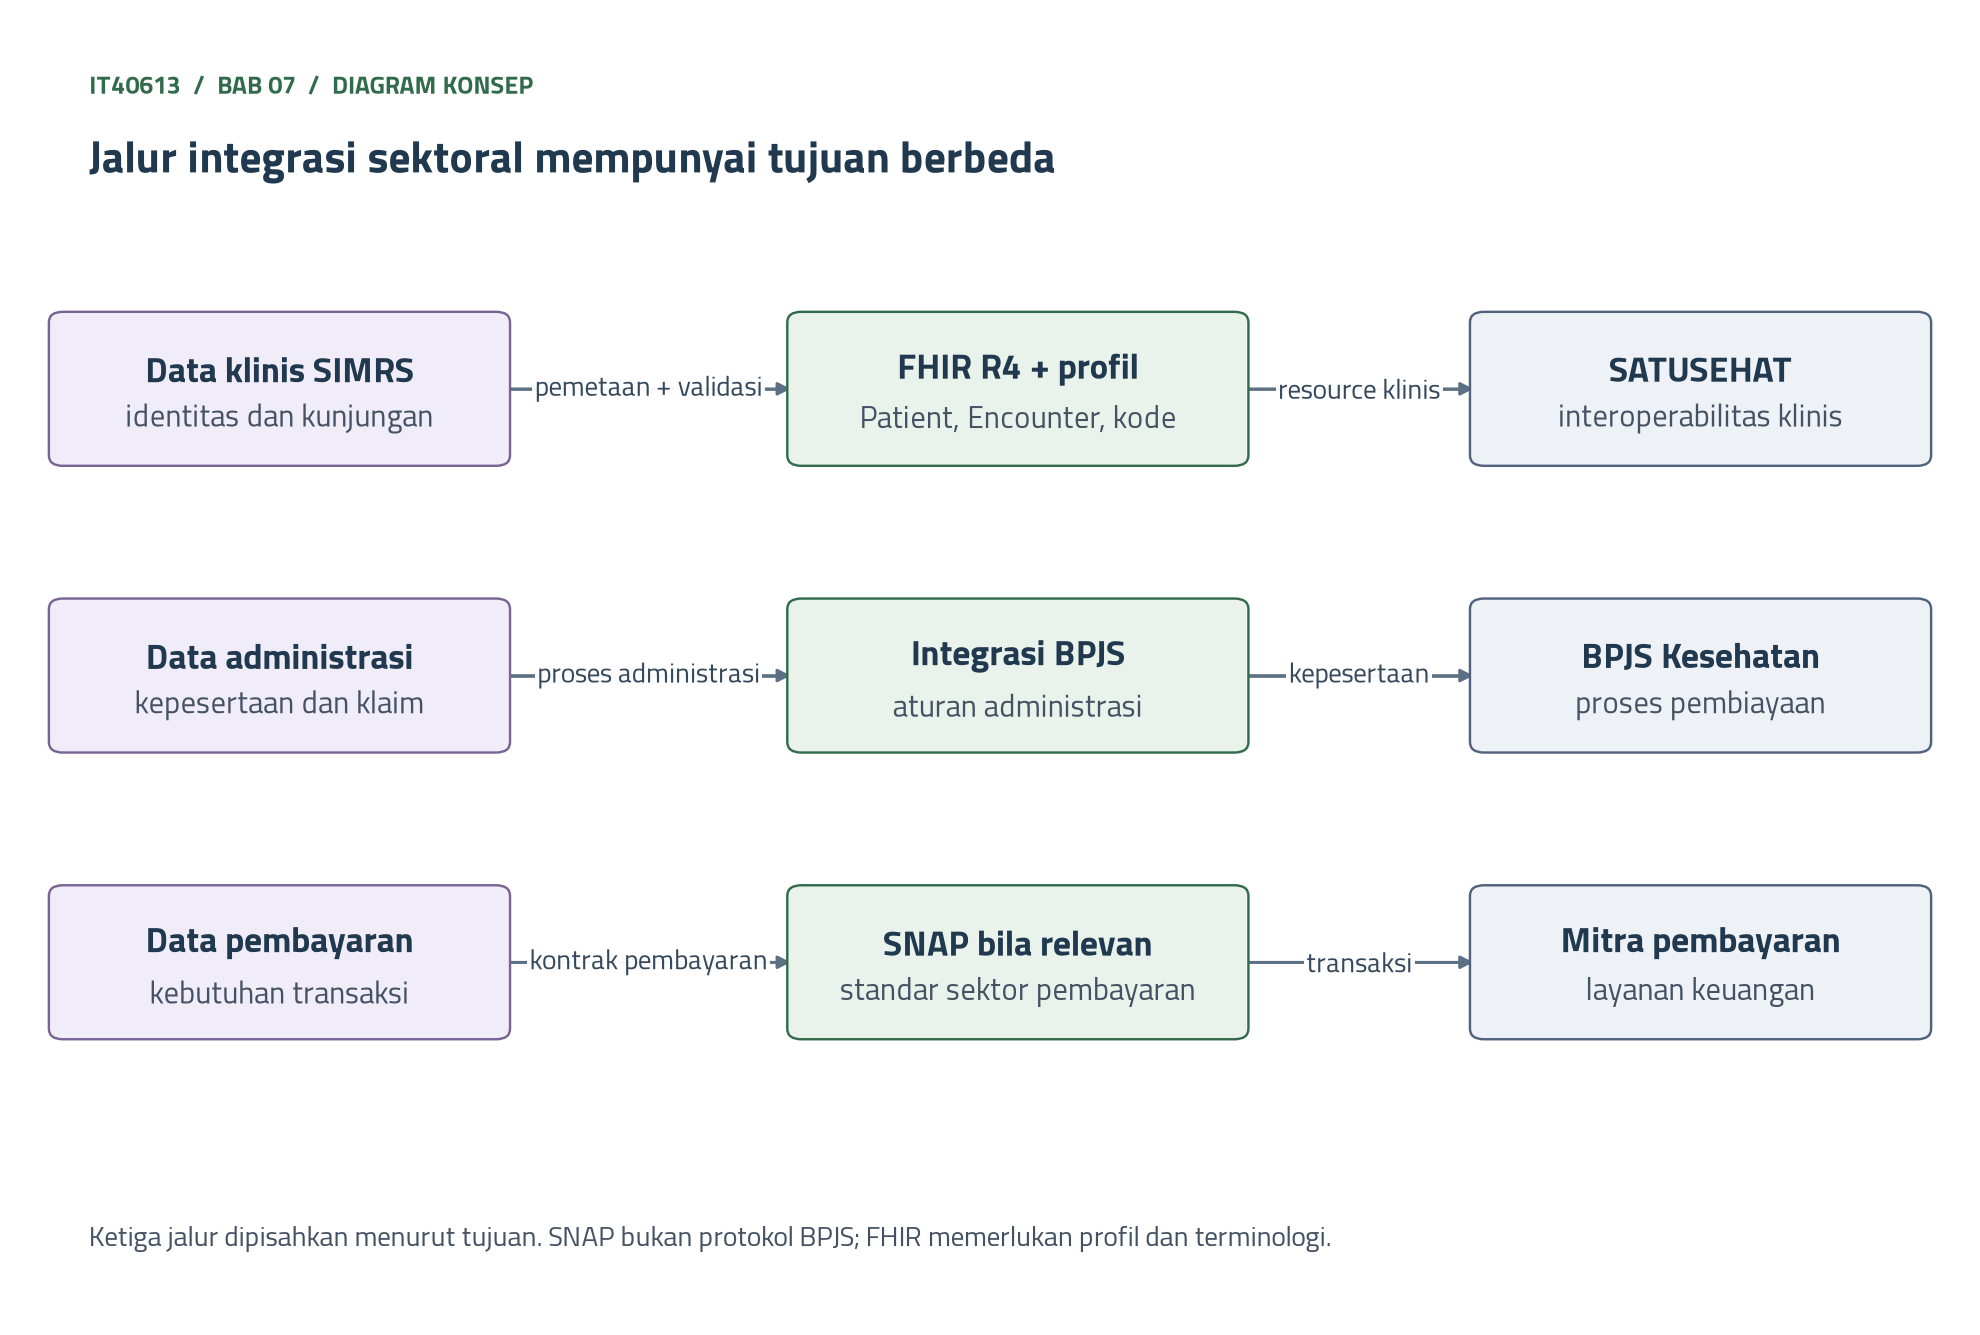
\includegraphics[width=0.96\textwidth,height=0.77\textheight,keepaspectratio]{../../figures/ch07-diagram-konsep.png}
\end{frame}

\section{Alasan Regulator}

\begin{frame}{{\Large Standar Mengurangi Penyepakatan Berulang}}
  \vspace{8pt}
  \begin{itemize}
    \item Tiap pihak memetakan data satu kali ke standar, bukan ke setiap mitra.
    \item Pasar dapat tertahan pada standar lama karena tiap pihak menunggu pihak lain: \textit{excess inertia}.
    \item Regulator memutus penantian dengan satu acuan dan satu tenggat.
    \item Standar tidak menghapus tata kelola. Organisasi tetap menjawab kebenaran, kelengkapan, dan kewenangan pengiriman data.
  \end{itemize}
  \vspace{6pt}
  {\small Analogi: kontainer baku memudahkan pemindahan, tetapi isi dan dokumen muatannya tetap diperiksa.}
\end{frame}

\begin{frame}{{\Large Empat Lapis Interoperabilitas}}
  \centering
  \eadiagram{../../figures/ch07-lapis-interoperabilitas.tex}
\end{frame}

\begin{frame}{{\Large Dua Contoh Berangka}}
  \vspace{8pt}
  \begin{itemize}
    \item Misalkan 18 klinik dan 5 rumah sakit menyepakati format per pasangan: 90 kesepakatan, Rp1,08 miliar.
    \item Dengan satu kontrak bersama: 23 pemetaan, Rp276 juta, pada Rp12 juta per pekerjaan.
    \item Misalkan 1 persen dari 100.000 kunjungan per bulan memuat kode sah yang keliru dipilih: 1.000 rekam lolos pemeriksaan format.
    \item Misalkan tim reviu memeriksa 200 rekam sampel, 6 menit per rekam: 20 jam, Rp1,2 juta per bulan.
  \end{itemize}
\end{frame}

\begin{frame}{{\Large Tiga Sumber Kewajiban}}
  \footnotesize
  \begin{tabularx}{\textwidth}{>{\raggedright\arraybackslash}p{2.1cm}
      >{\raggedright\arraybackslash}X >{\raggedright\arraybackslash}X >{\raggedright\arraybackslash}X}
    \hline
    \textbf{Sumber} & \textbf{Contoh} & \textbf{Akibat bila tidak dipenuhi} & \textbf{Ruang keputusan} \\ \hline
    Aturan hukum & Permenkes 24/2022 & Sanksi Pasal 42: teguran tertulis dan/atau rekomendasi pencabutan atau pencabutan status akreditasi & Cara menyambung, bukan apakah tersambung \\ \hline
    Syarat layanan & Peraturan BPJS Kesehatan 7/2018 & Kelengkapan klaim tidak terpenuhi & Alur internal dan pilihan vendor \\ \hline
    Pilihan bisnis & FHIR untuk 40 klinik mitra, API bank INT-08 & Tidak ada sanksi, ada biaya peluang & Bebas, setelah dihitung \\ \hline
  \end{tabularx}

  \vspace{8pt}
  \small Biaya mengikuti pihak wajib: 20 pekerjaan pembaruan, Rp240 juta per tahun. Lewat satu titik: 4 pekerjaan, Rp48 juta.
\end{frame}

\section{HL7 FHIR}

\begin{frame}{{\Large Resource, Profil, dan Terminologi}}
  \vspace{8pt}
  \begin{itemize}
    \item \textit{Resource}: unit dasar. Semua isi yang dapat dipertukarkan didefinisikan sebagai \textit{resource}.
    \item Patient memuat data pasien. Encounter memuat interaksi pasien dan penyedia layanan.
    \item Profil mempersempit aturan dasar untuk konteks implementasi.
    \item Terminologi menetapkan nilai kode yang sah dan maknanya.
  \end{itemize}
  \vspace{6pt}
  {\small Analogi: formulir baku punya kolom umum, aturan instansi menentukan kolom wajib dan daftar pilihan.}
\end{frame}

\begin{frame}{{\Large Hubungan Resource pada Satu Kunjungan}}
  \centering
  \eadiagram{../../figures/ch07-anatomi-fhir.tex}
\end{frame}

\begin{frame}{{\Large Tiga Konsep dan Cara Memeriksanya}}
  \footnotesize
  \begin{tabularx}{\textwidth}{>{\raggedright\arraybackslash}p{1.9cm}
      >{\raggedright\arraybackslash}X >{\raggedright\arraybackslash}X >{\raggedright\arraybackslash}X}
    \hline
    \textbf{Konsep} & \textbf{Pertanyaan} & \textbf{Contoh} & \textbf{Tanda kegagalan} \\ \hline
    \textit{Resource} & Objek apa yang dipertukarkan? & Patient dan Encounter adalah objek berbeda & Rekam pasien dibuat ulang setiap kunjungan \\ \hline
    Profil & Aturan tambahan apa yang berlaku di tujuan? & \texttt{Patient.identifier} boleh kosong pada aturan dasar, wajib di SATUSEHAT & JSON sah, tetapi ditolak penerima \\ \hline
    Terminologi & Nilai apa yang sah? & \texttt{Patient.gender} hanya menerima empat kode & Sistem Informasi Manajemen Rumah Sakit (SIMRS) mengirim \texttt{L} dan \texttt{P} tanpa pemetaan \\ \hline
  \end{tabularx}

  \vspace{8pt}
  \small SATUSEHAT: ICD-10 untuk diagnosis, ICD-9 CM untuk tindakan, LOINC untuk uji laboratorium, SNOMED CT untuk istilah klinis.
\end{frame}

\begin{frame}{{\Large Format Sah, Belum Tentu Sesuai Profil}}
  \vspace{8pt}
  \begin{itemize}
    \item Sah sebagai format: struktur JSON benar. Sesuai profil: aturan tujuan terpenuhi.
    \item \texttt{Patient.identifier} dan \texttt{Patient.name} 0..* pada R4, wajib menurut panduan SATUSEHAT.
    \item Misalkan 1,2 juta kunjungan dari 300.000 pasien. Bila tiap kunjungan membuat Patient baru: 900.000 rekam ganda.
    \item Misalkan kode lokasi kosong pada 2 persen dari 100.000 kiriman per bulan: 2.000 kiriman, sekitar 167 jam, Rp10 juta per bulan.
    \item Memperbaiki pemetaan di sumber dikerjakan satu kali.
  \end{itemize}
\end{frame}

\begin{frame}{{\Large Status R4, R5, dan R6}}
  \footnotesize
  \begin{tabularx}{\textwidth}{>{\raggedright\arraybackslash}p{1.0cm}
      >{\raggedright\arraybackslash}p{1.9cm} >{\raggedright\arraybackslash}X >{\raggedright\arraybackslash}X}
    \hline
    \textbf{Rilis} & \textbf{Versi, tahun} & \textbf{Status} & \textbf{Arti bagi Medikara} \\ \hline
    R4 & 4.0.1, 2019 & Campuran normatif dan \textit{trial use}, Patient normatif & Dipakai panduan implementasi SATUSEHAT \\ \hline
    R4B & 4.3.0, 2022 & Rilis antara pada area tertentu & Tidak diadopsi sebelum tujuan memintanya \\ \hline
    R5 & 5.0.0, 2023 & Sudah terbit, \textit{trial use}, sejumlah \textit{resource} dihapus atau diganti nama & Migrasi bukan sekadar menaikkan nomor versi \\ \hline
    R6 & 6.0.0, 2026 & Balot normatif, belum rilis final & Dipantau, belum dipakai untuk kiriman nyata \\ \hline
  \end{tabularx}

  \vspace{8pt}
  \small Status per 31 Oktober 2026. Misalkan migrasi Rp12 juta per sambungan: 5 sambungan INT-02 menghabiskan Rp60 juta tanpa kiriman yang lebih diterima.
\end{frame}

\section{SATUSEHAT}

\begin{frame}{{\Large SATUSEHAT dan Persiapan Kiriman}}
  \vspace{8pt}
  \begin{itemize}
    \item SATUSEHAT Platform menghubungkan sistem fasilitas, regulator, penjamin, dan penyedia layanan digital.
    \item Empat langkah persiapan: autentikasi, struktur organisasi, struktur lokasi, dan nomor IHS tenaga kesehatan.
    \item Nomor IHS pasien diperoleh dari \textit{Master Patient Index} (MPI).
    \item Encounter didaftarkan lebih dahulu. Rawat jalan sampai langkah 29, yaitu Composition untuk resume medis.
    \item Waktu dikirim dalam UTC+00: pukul 08.15 WIB ditulis 01:15.
  \end{itemize}
  \vspace{4pt}
  {\small Analogi: formulir yang benar sekaligus nomor rujukan yang dapat dikenali.}
\end{frame}

\begin{frame}{{\Large Pasal Permenkes 24/2022 yang Dibaca Tim}}
  \footnotesize
  \begin{tabularx}{\textwidth}{>{\raggedright\arraybackslash}p{1.1cm}
      >{\raggedright\arraybackslash}X >{\raggedright\arraybackslash}X}
    \hline
    \textbf{Pasal} & \textbf{Isi pokok} & \textbf{Arti bagi Medikara} \\ \hline
    3 & Setiap fasilitas wajib, termasuk klinik, rumah sakit, apotek, laboratorium & 5 rumah sakit, 18 klinik, 1 laboratorium, 12 apotek masuk cakupan \\ \hline
    21 & Harus terhubung dengan platform yang dikelola Kementerian Kesehatan & INT-02 hanya dapat dirapikan \\ \hline
    28 & Membuka akses seluruh isi rekam medis elektronik ke Kementerian Kesehatan & Dasarnya kewajiban, bukan persetujuan per kiriman \\ \hline
    34 & Persetujuan untuk administrasi dan jaminan pembiayaan saat registrasi & Periksa alur 55.000 kunjungan BPJS Kesehatan per bulan \\ \hline
    42 & Sanksi atas pelanggaran Pasal 3 & Risikonya menyentuh akreditasi \\ \hline
    45 & Tenggat 31 Desember 2023 & Kesenjangan adalah pekerjaan tertunda \\ \hline
  \end{tabularx}
\end{frame}

\begin{frame}{{\Large Alur Kiriman dan Titik Gagalnya}}
  \centering
  \eadiagram{../../figures/ch07-alur-satusehat.tex}
\end{frame}

\begin{frame}{{\Large Kasus: INT-02 Gagal Senyap (Data Latihan)}}
  \footnotesize
  \begin{tabularx}{\textwidth}{>{\raggedright\arraybackslash}X
      >{\raggedright\arraybackslash}p{1.4cm} >{\raggedright\arraybackslash}X}
    \hline
    \textbf{Penyebab (pemisalan)} & \textbf{Kiriman} & \textbf{Yang menyelesaikan} \\ \hline
    Identitas pasien belum cocok dengan MPI & 1.800 & Pencocokan saat registrasi \\ \hline
    Kode lokasi atau organisasi salah & 1.000 & Pendaftaran data induk \\ \hline
    Kode diagnosis lokal & 600 & Peta kode oleh koder \\ \hline
    Koneksi, token, atau waktu habis & 600 & Antrean kirim ulang \\ \hline
    \textbf{Jumlah per bulan} & \textbf{4.000} & \\ \hline
  \end{tabularx}

  \vspace{8pt}
  \small Misalkan 4 persen berlaku pada seluruh kiriman. Kirim ulang hanya menyelesaikan 15 persen. Tanpa rekonsiliasi, tumpukan 48.000 kiriman per tahun: 4.000 jam, Rp240 juta. Inventaris mencatat 0 jam manual: biayanya tidak terlihat, bukan tidak ada.
\end{frame}

\section{BPJS Kesehatan}

\begin{frame}{{\Large BPJS Kesehatan: Tujuannya Lain}}
  \vspace{8pt}
  \begin{itemize}
    \item INT-01 membawa kepesertaan, surat eligibilitas peserta (SEP), dan klaim.
    \item Peraturan BPJS Kesehatan 7/2018: lembar SEP bagian kelengkapan klaim (Pasal 19), dokumen dapat diminta lewat transaksi data elektronik (Pasal 28).
    \item Proses pembiayaan tidak identik dengan pertukaran klinis SATUSEHAT.
    \item Kepesertaan berbeda dari pembukaan isi rekam medis: persetujuan untuk klaim dicatat saat registrasi (Permenkes 24/2022 Pasal 34 ayat (7)).
  \end{itemize}
  \vspace{4pt}
  {\small Analogi: tiket perjalanan dan kuitansi berkaitan, tetapi menjawab pertanyaan berbeda.}
\end{frame}

\begin{frame}{{\Large Contoh Berangka pada INT-01}}
  \vspace{8pt}
  \begin{itemize}
    \item Dari 100.000 kunjungan per bulan, 55.000 juga melewati INT-01, atau 55 persen.
    \item Misalkan 1 persen punya data diri berbeda antara kartu dan SIMRS: 550 kunjungan, sekitar Rp2,75 juta per bulan.
    \item Misalkan 25 hari dan 10 jam layanan: 220 kunjungan per jam.
    \item Gangguan 2 jam menyisakan 440 kunjungan untuk diperiksa ulang: sekitar 37 jam, sekitar Rp2,2 juta.
    \item Prosedur sementara menjaga layanan pasien, lalu rekonsiliasi setelah pulih.
  \end{itemize}
\end{frame}

\begin{frame}{{\Large Tiga Jalur Mempunyai Tujuan Berbeda}}
  \footnotesize
  \begin{tabularx}{\textwidth}{>{\raggedright\arraybackslash}p{1.9cm}
      >{\raggedright\arraybackslash}X >{\raggedright\arraybackslash}X >{\raggedright\arraybackslash}p{2.7cm}}
    \hline
    \textbf{Jalur} & \textbf{Data} & \textbf{Acuan} & \textbf{Baris} \\ \hline
    Klinis & Identitas dan kunjungan, diagnosis, tindakan & FHIR R4, profil dan terminologi SATUSEHAT & INT-02, Manajer Rekam Medis \\ \hline
    Administrasi & Kepesertaan, SEP, dan klaim & Aturan dan spesifikasi BPJS Kesehatan & INT-01, Manajer Klaim \\ \hline
    Pembayaran & Mutasi dan kebutuhan transaksi & SNAP bila relevan, kontrak bank & INT-08, Manajer Keuangan \\ \hline
  \end{tabularx}

  \vspace{8pt}
  \small Jalur mulai bertemu: modul klaim BPJS di SATUSEHAT memakai ID Encounter, masih dalam pengembangan. Misalkan berlaku dengan kegagalan 4 persen: 2.200 klaim per bulan tanpa ID yang sah.
\end{frame}

\section{Open Banking dan SNAP}

\begin{frame}{{\Large Lima Istilah yang Sering Tertukar}}
  \footnotesize
  \begin{tabularx}{\textwidth}{>{\raggedright\arraybackslash}p{2.3cm}
      >{\raggedright\arraybackslash}p{2.6cm} >{\raggedright\arraybackslash}X}
    \hline
    \textbf{Istilah} & \textbf{Jenis} & \textbf{Yang dijawab} \\ \hline
    \textit{Open banking} & Konsep & Pemakaian bersama data nasabah yang diizinkan, dari bank ke pihak ketiga \\ \hline
    \textit{Open finance} & Konsep lebih luas & Ekosistem keuangan lebih luas, dengan API terstandar \\ \hline
    SNAP & Standar teknis nasional & Bentuk API pembayaran: protokol, autentikasi, enkripsi, struktur data \\ \hline
    POJK 21/2023 & Aturan bagi bank & Layanan digital oleh bank, sendiri atau bersama mitra \\ \hline
    PSD2 & Hukum Uni Eropa & Hak pengguna memakai layanan inisiasi pembayaran dan informasi rekening \\ \hline
  \end{tabularx}

  \vspace{6pt}
  {\small Analogi: standar colokan memudahkan penyambungan, tetapi izin pemakaian listrik punya aturan sendiri.}
\end{frame}

\begin{frame}{{\Large SNAP dan POJK 21/2023}}
  \vspace{8pt}
  \begin{itemize}
    \item SNAP: Keputusan Gubernur Bank Indonesia No.~23/10/KEP.GBI/2021, 16 Agustus 2021.
    \item Peraturan Anggota Dewan Gubernur (PADG) 23/15/PADG/2021 mewajibkan Penyedia Layanan dan Penyedia Jasa Pembayaran (PJP) Pengguna Layanan, tenggat bertahap 30 Juni 2022 sampai 30 Juni 2025.
    \item Asosiasi Sistem Pembayaran Indonesia (ASPI) mengelola sejak 1 September 2023. Versi 1.0.2: September 2024.
    \item Layanan: Registrasi, Informasi Saldo, Riwayat Transaksi, Transfer Kredit, Transfer Debit.
    \item POJK 21/2023: perjanjian kerja sama, akses data atas persetujuan, nasabah mengelola hak akses mitra.
  \end{itemize}
\end{frame}

\begin{frame}{{\Large Dua Rel yang Sering Dicampur}}
  \centering
  \eadiagram{../../figures/ch07-rantai-snap.tex}
\end{frame}

\begin{frame}{{\Large Standar Bentuk Pesan Tidak Menjawab Semua}}
  \vspace{8pt}
  \begin{itemize}
    \item Layanan pembayaran mitra tidak memberi akses otomatis ke seluruh rekening pengguna.
    \item Misalkan cicilan rawat inap lewat Medikara+ bagi 1.000 pasien: 1.000 catatan dasar akses, bukan satu izin umum.
    \item Misalkan 12.000 pembayaran digital per bulan, 0,1 persen terkirim dua kali: 12 pasien tertagih ganda.
    \item Pada 30 menit per penanganan: Rp360.000 per bulan, belum termasuk kepercayaan pasien.
    \item Kunci idempotensi dari Bab 5 menjawab masalah ini.
  \end{itemize}
\end{frame}

\begin{frame}{{\Large Kasus Medikara: Apakah SNAP Berlaku?}}
  \vspace{8pt}
  \begin{itemize}
    \item Medikara bukan PJP, sehingga kewajiban SNAP tidak jatuh langsung. Ini penalaran bab, bukan pendapat hukum.
    \item INT-08: mutasi dari 2 bank mitra, manual 50 jam per bulan, atau Rp36 juta per tahun.
    \item Dua antarmuka: Rp90 juta per tahun. Satu antarmuka, bila spesifikasi kedua bank sama: Rp45 juta per tahun.
    \item Dari jam kerja saja, API masih lebih mahal Rp9 juta per tahun. Keputusan Bab 4, rapikan, tetap masuk akal.
    \item Dapat berubah bila penutupan keuangan terhambat, atau portal unduhan dihentikan.
  \end{itemize}
\end{frame}

\section{Pelajaran Lintas Sektor}

\begin{frame}{{\Large Indonesia dan Uni Eropa}}
  \footnotesize
  \begin{tabularx}{\textwidth}{>{\raggedright\arraybackslash}p{2.2cm}
      >{\raggedright\arraybackslash}X >{\raggedright\arraybackslash}X >{\raggedright\arraybackslash}p{1.9cm}}
    \hline
    \textbf{Aspek} & \textbf{Indonesia} & \textbf{Uni Eropa} & \textbf{Hasil} \\ \hline
    Tujuan & Interoperabilitas Open API Pembayaran & Akses terkelola ke rekening daring dan persaingan layanan & Persamaan \\ \hline
    Dasar pengguna & Akses mitra berdasarkan persetujuan (POJK 21/2023) & Persetujuan eksplisit (PSD2 Pasal 66 dan 67) & Persamaan \\ \hline
    Bentuk & Standar teknis yang ditetapkan otoritas & Hak hukum, ditambah syarat antarmuka bagi bank & Perbedaan \\ \hline
    Pihak ketiga & Bersama mitra berdasarkan perjanjian kerja sama & Tidak boleh bergantung pada hubungan kontraktual & Perbedaan \\ \hline
  \end{tabularx}

  \vspace{6pt}
  {\small Kerangka Uni Eropa masih bergerak: kesepakatan paket PSR dan PSD3 pada November 2025. Periksa status terbaru.}
\end{frame}

\begin{frame}{{\Large Yang Ditiru adalah Prinsip, Bukan Pasal}}
  \vspace{8pt}
  \begin{itemize}
    \item Pengguna mengelola izin sendiri: POJK 21/2023 dan paket pembayaran Uni Eropa.
    \item Spesifikasi terdokumentasi: Regulasi 2018/389 Pasal 30.
    \item Uji kesesuaian sebelum terhubung: 2 jam atau Rp120.000 saat ditinjau, 160 jam atau Rp9,6 juta sesudah 40 klinik mitra terhubung.
    \item Misalkan ``tanpa kontrak'' disalin ke INT-05: 9 asuransi tidak terikat, 468 klaim ditolak per bulan tetap perlu perundingan.
  \end{itemize}
  \vspace{4pt}
  {\small Analogi: pedoman keselamatan penerbangan mengilhami rumah sakit tanpa membuatnya tunduk pada aturan pesawat.}
\end{frame}

\section{Menilai Kesenjangan}

\begin{frame}{{\Large Skala Penilaian Kesenjangan}}
  \small
  \begin{tabularx}{\textwidth}{>{\raggedright\arraybackslash}p{2.5cm}
      >{\raggedright\arraybackslash}p{1.6cm} >{\raggedright\arraybackslash}X}
    \hline
    \textbf{Tingkat} & \textbf{Skor} & \textbf{Syarat} \\ \hline
    Terpenuhi & 2 & Ada bukti terverifikasi bahwa kewajiban berjalan \\ \hline
    Sebagian & 1 & Sebagian lingkup, atau penyebab kegagalan masih hipotesis \\ \hline
    Belum & 0 & Tidak berjalan, atau belum diperiksa \\ \hline
    Tidak berlaku & Tidak dihitung & Ada alasan tertulis \\ \hline
  \end{tabularx}

  \vspace{8pt}
  Bukan audit kepatuhan, bukan pendapat hukum. Skala disusun bab ini.

  \vspace{4pt}
  {\small Analogi: kendaraan yang remnya belum diperiksa tidak dianggap lulus uji kelaikan.}
\end{frame}

\begin{frame}{{\Large Peta Keputusan}}
  \centering
  \eadiagram{../../figures/ch07-peta-keputusan.tex}
\end{frame}

\begin{frame}{{\Large Kasus Medikara: Penilaian Kesiapan}}
  \scriptsize
  \begin{tabularx}{\textwidth}{>{\raggedright\arraybackslash}p{0.8cm}
      >{\raggedright\arraybackslash}p{1.15cm} >{\raggedright\arraybackslash}X >{\raggedright\arraybackslash}X
      >{\raggedright\arraybackslash}p{1.25cm} >{\raggedright\arraybackslash}p{1.65cm}}
    \hline
    \textbf{ID} & \textbf{Baris} & \textbf{Kewajiban} & \textbf{Kondisi} & \textbf{Tingkat} & \textbf{Bukti} \\ \hline
    KI-01 & INT-02 & Kiriman lengkap & 4 persen belum terkirim & Sebagian & Terverifikasi \\ \hline
    KI-02 & INT-02 & Status kiriman tertelusuri & Gagal tanpa pemberitahuan & Belum & Terverifikasi \\ \hline
    KI-03 & INT-02 & Identitas dan data induk cocok & Misalkan 2.800 gagal per bulan & Sebagian & Hipotesis \\ \hline
    KI-04 & INT-02 & Terminologi yang ditetapkan & Misalkan 600 gagal per bulan & Sebagian & Hipotesis \\ \hline
    KI-05 & INT-09, INT-10 & 18 klinik, 1 laboratorium, 12 apotek & Jalur belum tercatat & Belum & Belum terverifikasi \\ \hline
    KI-06 & INT-01 & Kepesertaan, SEP, klaim & 5 sambungan berjalan & Terpenuhi & Terverifikasi \\ \hline
    KI-07 & INT-01 & Persetujuan saat registrasi & Belum diperiksa & Belum & Belum terverifikasi \\ \hline
    KI-08 & INT-08 & SNAP & Medikara bukan PJP & Tidak berlaku & Terverifikasi \\ \hline
  \end{tabularx}
\end{frame}

\begin{frame}{{\Large Membaca Skor dan Menentukan Prioritas}}
  \vspace{8pt}
  \begin{itemize}
    \item Tujuh baris berlaku: skor 5 dari 14, sekitar 36 persen.
    \item Baris terverifikasi saja: 3 dari 6, atau 50 persen. Selisihnya adalah pengetahuan yang belum ada.
    \item KI-02 lebih dahulu: Misalkan 1 jam per hari, Rp18 juta per tahun, dibanding sekitar Rp240 juta bila dibiarkan.
    \item KI-05 dan KI-07 diperiksa, KI-03 dan KI-04 diuji lewat sampel kiriman gagal.
    \item Skor selalu disajikan bersama daftar barisnya.
  \end{itemize}
\end{frame}

\section{Aktivitas}

\begin{frame}{{\Large Aktivitas: Tujuan dan Peran}}
  \vspace{6pt}
  \begin{itemize}
    \item Tujuan: menilai kesenjangan integrasi terhadap standar sektor, menjadi artefak C2 yang dapat ditelusuri.
    \item Medikara: SATUSEHAT dan BPJS Kesehatan. Organisasi keuangan: SNAP.
    \item Latar kesehatan, hukum, atau keuangan: membaca kewajiban beserta tenggatnya.
    \item Latar teknis: membandingkan data yang dikirim dengan \textit{resource} atau spesifikasi.
    \item Latar bisnis atau akuntansi: menghitung dampak layanan dan biaya.
  \end{itemize}
  \vspace{4pt}
  {\small Data organisasi nyata seizin organisasi dan dianonimkan. Data pribadi pasien atau karyawan tidak boleh dipakai.}
\end{frame}

\begin{frame}{{\Large Aktivitas: Langkah dan Luaran}}
  \vspace{4pt}
  \begin{enumerate}
    \item Pilih satu sampai tiga baris inventaris Bab 4, tandai jalurnya.
    \item Tulis standar yang berlaku beserta pasal atau dokumen dasarnya.
    \item Petakan satu alur data ke \textit{resource} dan profil tujuan.
    \item Catat kesenjangan pada empat lapis, beri tingkat dan status bukti.
    \item Tetapkan pemilik, tindakan, dan tanggal tinjau.
  \end{enumerate}
  \vspace{4pt}
  {\small Luaran: lembar penilaian, ringkasan satu halaman, catatan alternatif, tautan bukti. Melengkapi C2 menjelang UTS. Bobot: konsep 25, bukti 30, alasan 30, keterbacaan 15 persen. Berkas: \texttt{sources/chapter07/}.}
\end{frame}

\section{Ringkasan dan Latihan}

\begin{frame}{{\Large Ringkasan}}
  \vspace{6pt}
  \begin{itemize}
    \item Standar mengurangi penyepakatan berulang, tetapi tidak menghapus tata kelola.
    \item FHIR: \textit{resource}, profil, dan terminologi. JSON sah dapat tetap ditolak.
    \item SATUSEHAT dan BPJS Kesehatan menjalankan tujuan berbeda. SNAP bukan protokol BPJS.
    \item Medikara bukan PJP, dan hitungan INT-08 belum memihak API. Prinsip lintas sektor ditiru, pasalnya tidak.
    \item Skor sekitar 36 persen adalah peta pekerjaan dan peta ketidaktahuan, bukan nilai kepatuhan.
  \end{itemize}
\end{frame}

\begin{frame}{{\Large Latihan 1: Menilai Manfaat Standar Terbuka}}
  \vspace{8pt}
  Jelaskan mengapa SATUSEHAT memakai standar terbuka seperti HL7 FHIR, bukan format buatan sendiri.
  \vspace{6pt}
  \begin{itemize}
    \item Pilih satu pertukaran data klinis.
    \item Bandingkan format lokal dengan FHIR pada empat lapis.
    \item Hitung jumlah pemetaan pada kedua pilihan.
    \item Jelaskan manfaat dan batas standardisasi.
  \end{itemize}
  \vspace{4pt}
  {\small Pembanding: 90 kesepakatan, Rp1,08 miliar, dan 23 pemetaan, Rp276 juta.}
\end{frame}

\begin{frame}{{\Large Latihan 2: Membandingkan SNAP dan PSD2}}
  \vspace{8pt}
  Bandingkan cara Indonesia melalui SNAP dan Uni Eropa melalui PSD2 mendorong \textit{open banking}. Sebutkan satu persamaan dan satu perbedaan.
  \vspace{6pt}
  \begin{itemize}
    \item Tentukan cakupan dan pihak setiap kerangka.
    \item Cari sumber resmi, lalu catat nomor pasal.
    \item Pisahkan persamaan prinsip dari perbedaan hukum.
    \item Tentukan satu standar yang relevan bagi organisasi tim.
  \end{itemize}
\end{frame}

\begin{frame}{{\Large Latihan 3: Mendiagnosis Pengiriman yang Gagal}}
  \vspace{8pt}
  Misalkan data kunjungan pasien dari dua rumah sakit Medikara belum terkirim ke SATUSEHAT. Uraikan tiga kemungkinan penyebab dari sisi proses, data, dan teknologi.
  \vspace{6pt}
  \begin{itemize}
    \item Contoh: Bogor dan Bandung, 30.000 kunjungan per bulan, 14 hari, 14.000 kiriman.
    \item Ajukan sebab proses, data, dan teknologi.
    \item Tentukan bukti untuk menguji setiap dugaan.
    \item Tentukan dugaan pertama dan bukti keberhasilan perbaikan.
  \end{itemize}
\end{frame}

\end{document}
